\documentclass{standalone}
\usepackage{tikz}
 \usetikzlibrary{decorations.pathreplacing} %

\begin{document}
		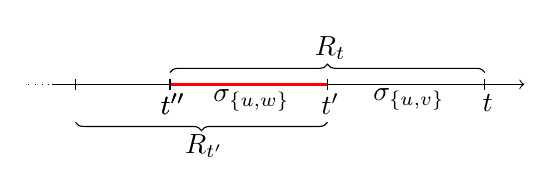
\begin{tikzpicture}
	\draw [->] (-10mm,0) -- (5,0);
	\draw [dotted] (-13mm,0) -- (-10mm,0);
	
	\draw [decorate,decoration={brace,amplitude=3pt}] (5mm,0.15) -- (45mm,0.15)
	node [black,midway,above=1pt,xshift=1pt] {$R_{t}$};
	
	\draw [decorate,decoration={brace,amplitude=3pt}, yshift=-18pt] (25mm,0.15) -- (-7mm,0.15)
	node [black,midway,below=1pt,xshift=1pt] {$R_{t'}$};
	
	\draw [] (45mm,2pt) -- (45mm,-2pt)
	node [black,midway,below=0pt,xshift=1pt] {$t$};
	
	% tick
	\draw [] (25mm,2pt) -- (25mm,-2pt)
	node [black,midway,below=0pt,xshift=1pt] {$t'$};
	% tick
	\draw [] (5mm,2pt) -- (5mm,-2pt)
	node [black,midway,below=0pt,xshift=1pt] {$t''$};
	% tick
	\draw [] (-7mm,2pt) -- (-7mm,-2pt)
	node [black,midway,below=0pt,xshift=1pt] {};
	
	\draw [line width=0.33mm, red] (5mm,0) -- (25mm,0) 
	node [black,midway,below=-2pt,xshift=1pt] {$\sigma_{\{u,w\}}$};
	
	\draw [] (25mm,0) -- (45mm,0) 
	node [black,midway,below=-2pt,xshift=1pt] {$\sigma_{\{u,v\}}$};
	
	\draw [] (5mm,2pt) -- (5mm,-2pt)
	node [black,midway,below=0pt,xshift=1pt] {$t''$};
	%% vertical arrow 
	%\draw [->] (3mm,14pt) -- (4.4mm,4pt)
	%node [black,midway,above=0pt,xshift=-4pt] {separation of  $\{u,w\}$};
	%% vertical arrow 
	%\draw [->] (30mm,-24pt) -- (26.5mm,-7pt)
	%node [black,midway,below=0pt,xshift=5pt, yshift=-5pt] {separation of  $\{u,v\}$};
	\end{tikzpicture}
	
\end{document}